\documentclass[12pt,fleqn, parskip=full]{scrartcl}

\usepackage{amsmath}
\usepackage{fancyhdr}
\usepackage{graphicx}
\usepackage{float}

\pagestyle{fancy}
\lhead{Donald Doyle UIN: 128005953}

\title{NUEN 301 \\
Homework 1}
\author{Donald Doyle UIN: 128005953}
\date{\today}

\begin{document}

\maketitle


Exercise 1 [20 pts]: [computing atom densities and macroscopic XS]\\
Compute the total, elastic, fission, and radiative capture macroscopic cross sections for $UO_2$ (4 types of macroscopic XS in total).\\
• Assume $UO_2$ is only made of U-235, U-238, and O-16. U-235 has been enriched at 25 weight\%. Density of $UO_2$ is $10.4$ [g/cc].\\
• We are interested in computing macroscopic cross sections for both the thermal range (Maximillian
average) and the fission spectrum range. Therefore, you will have to procedure 8 macroscopic cross
sections in total. \\
a. [7 pts] Fill the table below: \\
\begin{table}[H]
\small
\begin{center}
\resizebox{\textwidth}{!}{\begin{tabular}{|c|c|c|}
\hline
variable & value & unit \\
\hline
Molar mass of U-235 & 235.0439282 & g/mol \\
\hline
Molar mass of U-238 & 238.050787 & g/mol \\
\hline
Molar mass of O-16  & 15.99491462 & g/mol\\
\hline
Avogadro number & $6.0221409*10^{23}$ & atoms/mol\\
\hline
(n,total) microscopic XS for U-235 (Maxwellian average)  & 686.2 & b\\
\hline
(n,elastic) microscopic XS for U-235 (Maxwellian average)  & 16.95 & b\\
\hline
(n,fission) microscopic XS for U-235 (Maxwellian average)  & 571.4 & b\\
\hline
(n,$\gamma$) microscopic XS for U-235 (Maxwellian average)  & 97.83 & b\\
\hline
(n,total) microscopic XS for U-238 (Maxwellian average)  & 13.19 & b\\
\hline
(n,elastic) microscopic XS for U-238 (Maxwellian average)  & 10.50 & b\\
\hline
(n,fission) microscopic XS for U-238 (Maxwellian average)  & $1.683*10^{-5}$ & b\\
\hline
(n,$\gamma$) microscopic XS for U-238 (Maxwellian average)  & 2.690 & b\\
\hline
(n,total) microscopic XS for O-16 (Maxwellian average)  & 4.474 & b\\
\hline
(n,elastic) microscopic XS for O-16 (Maxwellian average)  & 4.474 & b\\
\hline
(n,fission) microscopic XS for O-16 (Maxwellian average)  & 0 & b\\
\hline
(n,$\gamma$) microscopic XS for O-16 (Maxwellian average)  & $1.9*10^{-4}$ & b\\
\hline
(n,total) microscopic XS for U-235 (fission spectrum average)  & 7.628 & b\\
\hline
(n,elastic) microscopic XS for U-235 (fission spectrum average)  & 4.451 & b\\
\hline
(n,fission) microscopic XS for U-235 (fission spectrum average)  & 1.218 & b\\
\hline
(n,$\gamma$) microscopic XS for U-235 (fission spectrum average)  & 0.08741 & b\\
\hline
(n,total) microscopic XS for U-238 (fission spectrum average)  & 7.759 & b\\
\hline
(n,elastic) microscopic XS for U-238 (fission spectrum average)  & 4.827 & b\\
\hline
(n,fission) microscopic XS for U-238 (fission spectrum average)  & 0.3064 & b\\
\hline
(n,$\gamma$) microscopic XS for U-238 (fission spectrum average)  & 0.07016 & b\\
\hline
(n,total) microscopic XS for O-16 (fission spectrum average)  & 2.764 & b\\
\hline
(n,elastic) microscopic XS for O-16 (fission spectrum average)  & 2.751 & b\\
\hline
(n,fission) microscopic XS for O-16 (fission spectrum average)  & 0 & b\\
\hline
(n,$\gamma$) microscopic XS for O-16 (fission spectrum average)  & $1.136*10^{-4}$ & b\\
\hline
\end{tabular}}
\end{center}
\end{table}

b. [4 pts] Compute the molar mass of $UO_2$. \\
$M_{H_2O} = \gamma M_{U-235} + (1 - \gamma) M_{U-238} + 2M_O = .25(235.0439282) + .75(238.050787) + 2(15.99491462) = 269.2889015$\\
c. [5 pts] Compute the atom densities for O-16, U-235, U-238.\\
$N_{U-235} = \frac{0.25(10.4)(6.0221409*10^23)}{235.0439282} = 6.661549*10^21 [atoms/cm^3]$\\

$N_{U-237} = \frac{0.75(10.4)(6.0221409*10^23)}{238.050787} = 1.973222*10^22 [atoms/cm^3]$\\

$N_{O-16} = \frac{2(10.4)(6.0221409*10^23)}{15.99491462} = 7.831272*10^23 [atoms/cm^3]$ \\


d. [4 pts] Compute the 8 requested macroscopic cross sections\\
$\Sigma_{total}$ (Maxwellian average) $ = (686.2)(10^{-24})(6.661549*10^21)+(13.19)(10^{-24})(1.973222*10^22)+(4.474)(10^{-24})(7.831272*10^23) = 4.693436359 [cm^-1]$\\

$\Sigma_{elastic}$ (Maxwellian average) $ = (16.95)(10^{-24})(6.661549*10^21)+(10.50)(10^{-24})(1.973222*10^22)+(4.474)(10^{-24})(7.831272*10^23) = 3.533098798 [cm^-1] $ \\

$\Sigma_{fission}$ (Maxwellian average)$  = (571.4 )(10^{-24})(6.661549*10^21)+(1.683*10^-5)(10^{-24})(1.973222*10^22)+(0)(10^{-24})(7.831272*10^23) = 0.990686414 [cm^-1]$\\

$\Sigma_{\gamma}$ (Maxwellian average) $ = (97.83)(10^{-24})(6.661549*10^21)+(2.690)(10^{-24})(1.973222*10^22)+(1.9*10^-4)(10^{-24})(7.831272*10^23) = 0.169765266 [cm^-1]$\\

$\Sigma_{total}$ (fission spectrum average) $ = (7.628)(10^{-24})(6.661549*10^21)+(7.759)(10^{-24})(1.973222*10^22)+(2.764)(10^{-24})(7.831272*10^23) = 2.177788915 [cm^-1]$\\

$\Sigma_{elastic}$ (fission spectrum average) $ = (4.451)(10^{-24})(6.661549*10^21)+(4.827)(10^{-24})(1.973222*10^22)+(2.751)(10^{-24})(7.831272*10^23) = 2.132100017 [cm^-1]$\\

$\Sigma_{fission}$ (fission spectrum average) $  = (1.218)(10^{-24})(6.661549*10^21)+(0.3064)(10^{-24})(1.973222*10^22)+(0)(10^{-24})(7.831272*10^23) = 0.002111754 [cm^-1]$\\

$\Sigma_{\gamma}$ (fission spectrum average) $ = (0.08741)(10^{-24})(6.661549*10^21)+(0.07016)(10^{-24})(1.973222*10^22)+(1.136*10^-4)(10^{-24})(7.831272*10^23) = 2.405136515*10^-4 [cm^-1]$\\


Exercise 2 [10 pts]: [on the meaning of microscopic XS]\\
a. [3 pts] Assume a homogeneous material made of U-235. Use the data collected in Exercise 1. What is the probability that the outcome of collision for an incident neutron of thermal energy (Maxwell average) is a\\
1. Fission\\
$\frac{16.95}{686.2} = 0.0247$\\

2. Radiative capture\\
$\frac{571.4}{686.2} = 0.8327$\\

3. Elastic Scattering\\
$\frac{97.83}{686.2} = 0.1426$\\

b. [3 pts] Repeat Question a) but assume that the neutron is a fast neutron (fission spectrum average)\\
$\frac{4.451}{7.628} = 0.5835$\\

$\frac{1.218}{7.628} = 0.1597$\\

$\frac{0.08741}{7.628} = 0.0115$\\

c. [2 pts] Now assume that the homogeneous material is O-16. What is the most probable outcome of a collision on O-16 if the incident neutron is thermal (Maxwell average). What is the probability for that
outcome?\\
The most likely  event is elastic scattering $\frac{4.474}{4.474} = 1$\\

d. [2 pts] Still assuming that the homogeneous material is O-16. What are the two most probable outcome of a collision on O-16 if the incident neutron is fast (fission spectrum average). What are the probabilities for these two outcomes?\\
The most likely  event is elastic scattering $\frac{2.751}{2.764} = 0.9953$\\

Exercise 3 [20 pts]: [computing atom densities and macroscopic XS]\\
A boiling water reactor operates at 1000 psi. At that pressure the density of water and of steam are, respectively, $0.74$ [g/cm3] and $0.036$ [g/cm3]. Use these entries in the database and pick the thermal (Maxwellian) average values.\\
a. [5 pts] What is the macroscopic total cross section of the water?\\
$\Sigma_{water} = \frac{(0.74)(6.0221409*10^{23})}{2(1.00794) + 15.9994}(2(33.15*10^{-24}) + (4.463*10^{-24})) = 1.750442512 [cm^-1]$\\

b. [5 pts] What is the macroscopic total cross section of the steam?\\
$\Sigma_{steam} = \frac{(0.036)(6.0221409*10^{23})}{2(1.00794) + 15.9994}(2(33.15*10^{-24}) + (4.463*10^{-24})) = 0.0851566628 [cm^-1]$\\

c. [5 pts] If, on average, 40% of the volume is occupied by steam, then what is the macroscopic total cross section of the steam–water mixture?\\
$\Sigma_{total} = .4(0.0851566628) + .6(1.750442512) = 1.084328172 [cm^-1]$\\

d. [5 pts] What is the macroscopic total cross section of water under atmospheric conditions at room
temperature?\\
$\Sigma_{water} = \frac{(1)(6.0221409*10^{23})}{2(1.00794) + 15.9994}(2(33.15*10^{-24}) + (4.463*10^{-24})) = 2.365462854 [cm^-1]$\\

Exercise 4 [25 pts]: [reaction rates for uncollided beam, think and thick target meanings]\\
A beam of neutrons of energy $E_1$ is normally incident on a homogeneous slab $3$ [cm] thick. The area of the slab covered by the beam is $6 [cm^2]$. The intensity of neutrons transmitted through the slab without interactions is found to be 25% of the incident intensity.\\
a. [2 pts] What is the total macroscopic cross section for the slab material at energy $E_1$?\\
$I(x) - I_0 e^{-\Sigma_t X} \Rightarrow \Sigma_t = \frac{-ln(.25)}{3} = 0.462098 [cm^-1]$\\

b. [2 pts] What is the average distance a neutron travels in this material before undergoing an interaction?\\
Mean free path $= \frac{1}{\Sigma_t} = \frac{1}{0.462098} = 2.16404 [cm]$\\

c. [2 pts] At another neutron energy $E_2$, the macroscopic cross section is found to be 50 times smaller than in (a). What is the fraction of neutrons of that energy that would be transmitted through the slab without interactions?\\
$\Sigma_t = \frac{0.462098}{50} = 0.00924196 [cm^-1] \Rightarrow I = I_0 e^{-0.00924196(3)} = 0.9727$\\ 

In what follows, assume the incident beam intensity to be $I_0(E_1) = I_0(E_2) = 10^6 [n/cm^2-s] $ \\
d. [4 pts] Compute the reaction rate in the slab using the thin-target approximation at both energies, $E_1$ and $E_2$.\\
$RR_{E_1} = I\Sigma_t = \Sigma IA\Delta x = (10^6)(0.462098)(6)(3) = 8317764 [reactions/s]\\
RR_{E_2} = I\Sigma_t = \Sigma IA\Delta x = (10^6)(0.00924196)(6)(3) = 166355 [reactions/s]$\\

e. [8 pts] Compute the reaction rate in the slab using the thick-target approximation at both energies, $E_1$ and $E_2$.\\
$RR_{E_1} = IA\frac{1-e^{-\Sigma L}}{\Sigma} = (10^6)(6)\frac{1-e^{-(0.462098)(3)}}{(0.462098)} = 9738163 [reactions/s]\\
RR_{E_1} = IA\frac{1-e^{-\Sigma L}}{\Sigma} = (10^6)(6)\frac{1-e^{-(0.00924196)(3)}}{(0.00924196)} = 17752757 [reactions/s]$\\

f. [2 pts] In which case is the thin target a good approximation? Provide the relative errors, at both energies, $E_1$ and $E_2$.\\
$Error_{E_1} = \frac{|8317764 - 9738163}{9738163}*100 = 14.5859\%\\
Error_{E_2} = \frac{|166355 - 17752757}{17752757}*100 = 99.0629\% $ \\

g. [1 pts] To further understand what is going on, write the Taylor Series expansion for the function   $f(x) = 1 - exp(-x)$ around zero.\\


h. [4 pts] Show that the thick-target expression for the reaction rate becomes the thin-target expression when “something” is small. What is that “something”?\\

Exercise 5 [25 pts]: [on the thermal motion of the target nucleus and the averaging of XS]\\
Consider a hypothetical material whose nuclei are moving with a velocity $\overrightarrow{V}$ as follows:\\
• all nuclei have speed $ V = ||\overrightarrow{V}|| = 10,000 [\frac{cm}{s}]$\\
• at any given time 1/5 of nuclei are moving in direction $+\hat{i}$\\
• at any given time 1/5 of nuclei are moving in direction $-\hat{i}$\\
• at any given time 3/5 of nuclei are at rest.\\
 Here $\hat{i} \hat{j} \hat{k}$ are unit vectors along the x, y, and z axes. Suppose the cold cross section for this material is as given in the following table and plot. Recall that the cold cross section is the cross section when there is no thermal motion.\\

\begin{figure}[H]
	\centering
	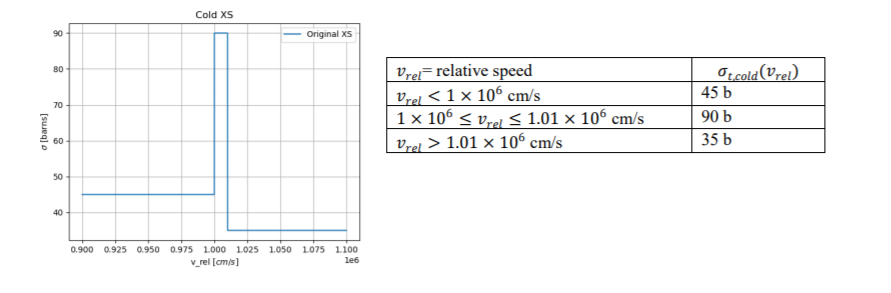
\includegraphics[scale=.7]{Image_1_hw_1}
\end{figure}

Consider a mono-directional beam of neutrons of intensity $I = n \times v_tab$ incident from the left on a thin slice of this material (neutrons are traveling along the x-axis, in direction $+\hat{i}$). This beam has a uniform lab-frame speed distribution, i.e., $ 0.95 × 106 \leq v_tab \leq 1.1 × 106 \frac{cm}{s}]$ Compute the appropriate averaged cross section for each neutron lab-frame speed and plot that average cross section on the same plot as the cold cross section.
\begin{figure}[H]
	\centering
	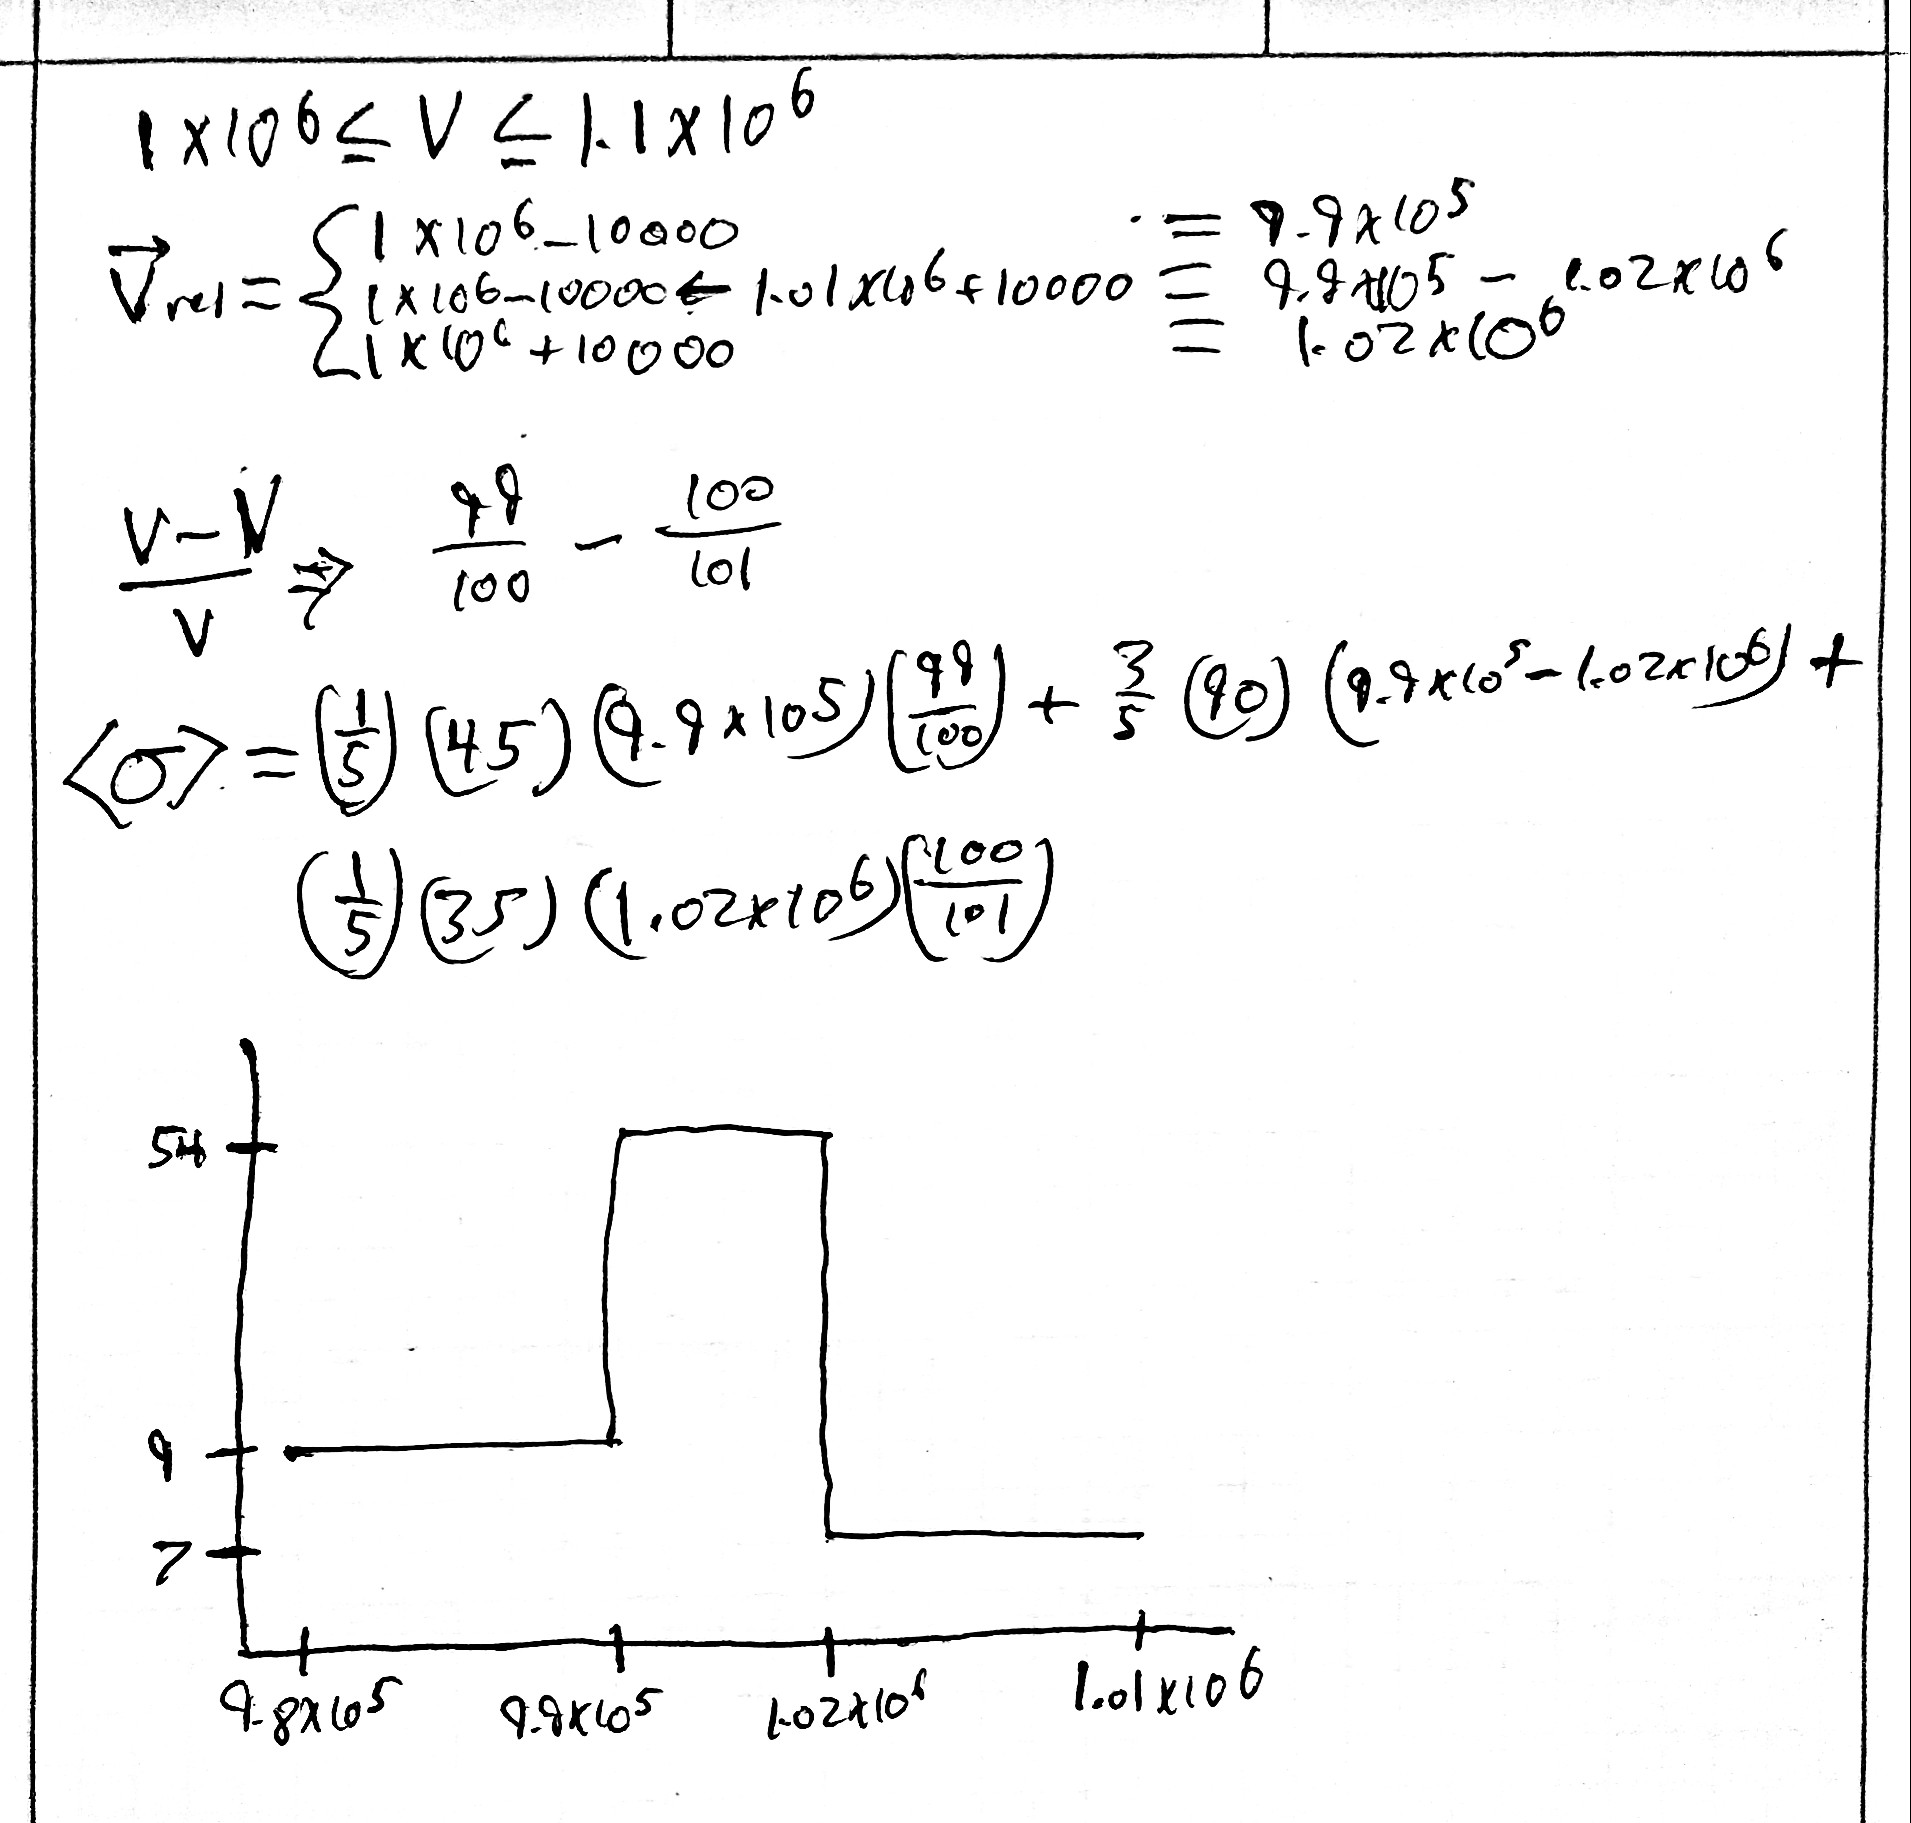
\includegraphics[scale=.2]{Image_2_hw_1}
\end{figure}

Exercise 6 [10 EXTRA pts, MADATORY for Honors]: [Monte Carlo]
Implement 2-stream scattering in your Monte Carlo code. Use the following values. $\Sigma_t = 10 [cm^-1]$, $\Sigma_a = 4 [cm^-1]]$, slab thickness = 0.5 cm. Normally incident beam on the left with intensity =1000.

\end{document}